%!TEX TS-program = xelatex
 
% Этот шаблон документа разработан в 2014 году
% Данилом Фёдоровых (danil@fedorovykh.ru) 
% для использования в курсе 
% <<Документы и презентации в \LaTeX>>, записанном НИУ ВШЭ
% для Coursera.org: http://coursera.org/course/latex .
% Исходная версия шаблона --- 
% https://www.writelatex.com/coursera/latex/5.2.2
 
\documentclass[a4paper,12pt]{article}
 
%%% Работа с русским языком
\usepackage[english,russian]{babel}   %% загружает пакет многоязыковой вёрстки
\usepackage{fontspec}      %% подготавливает загрузку шрифтов Open Type, True Type и др.
\defaultfontfeatures{Ligatures={TeX},Renderer=Basic}  %% свойства шрифтов по умолчанию
\setmainfont[Ligatures={TeX,Historic}]{Times New Roman} %% задаёт основной шрифт документа
\setsansfont{Comic Sans MS}                    %% задаёт шрифт без засечек
\setmonofont{Courier New}
\usepackage{indentfirst}
\frenchspacing
 
%%% Дополнительная работа с математикой
\usepackage{amsmath,amsfonts,amssymb,amsthm,mathtools} % AMS
\usepackage{icomma} % "Умная" запятая: $0,2$ --- число, $0, 2$ --- перечисление
 %% Номера формул
\mathtoolsset{showonlyrefs=true} % Показывать номера только у тех формул, на которые есть \eqref{} в тексте.

\author{Батарин Егор}
\title{Интерференция лазерного излучения}
\date{\today}
 
\begin{document} % конец преамбулы, начало документа
 
\maketitle
 
\begin{abstract}
   Цель работы: исследовать зависимость видности интерференционной картины от разности хода интерферирующих лучей и от их поляризации. Точнее говоря, нужно исследовать: 
а) характер поляризации лучей
в интерферометре; б) зависимость видности интерференционной
картины от угла
α между плоскостями поляризации интерферирующих волн
при нулевой разности
хода; в) зависимость видности интерференционной
картины от разности
хода интерферирующих лучей для угла $\alpha = 0$. По
результатам измерений следует оценить спектральные
характеристики
лазерного излучения.
\end{abstract}
\section{Теория}
\subsection{Видность интерференционной картины}
Для описания четкости интерференционной картины вводится видность:

\begin{equation}\label{eq:vindost}
\gamma = \frac{I_{max} - I_{min}}{I_{max}+I_{min}}
\end{equation}

Интенсивность для моды лазерного излучения с частотой $f_m$ интерференционной картины двух волн с амплитудами $A_m$ и $B_m$ имеет вид:

\begin{equation}\label{eq:intes}
I_m = A^2_m + B^2_m + 2A_mB_m\cos (k_ml)
\end{equation}
где волновое число $k_m = \frac{2\pi}{\lambda_m}$.
По формуле \eqref{eq:vindost} можно опрелелить видность интерференционной картины, где положено $\delta = \frac{B^2_m}{A^2_m}$.:
\begin{equation}\label{eq:vidnost2}
\gamma_1=\frac{2\sqrt{\delta}}{1+\delta}
\end{equation}


Интесивность нескольких мод лазерного излучения имеет вид:
\begin{equation}\label{eq:sumintes}
I = \sum\limits_m I_m = \sum\limits_m A^2_m\left[ 1 + \delta + 2\sqrt{\delta}\cos{\left(\frac{2\pi f_m}{c}l\right)}\right]
\end{equation}

Учтем теперь влияние спектрального состава света на видность интерференционной картины. Для упрощения выкладок мы предположим, что частота наиболее интенсивной моды совпадает с центром доплеровского
контура $f_0$, а симметричные относительно $f_0$ моды имеют одинаковую амплитуду. В этом случае можно записать:
\begin{equation}\label{eq:freq}
f_m = f_0 + n\Delta\nu; \quad A^2_n = A^2_{-n}; \quad n = 0, \pm 1, \pm 2, ...
\end{equation}
Подставляя \eqref{eq:freq} в \eqref{eq:sumintes}, получим:
\begin{equation}\label{eq:sumintes2}
I =  \sum\limits_n A^2_n\left[ 1 + \delta + 2\sqrt{\delta}\cos{\left(\frac{2\pi f_n}{c}l\right)}\cos{\left(\frac{2\pi\Delta\nu}{c}n l\right)}\right]
\end{equation}
Поэтому, видность равна $\gamma = \gamma_1\gamma_2$, где
\begin{equation}\label{eq:gamma2}
\gamma_2(l) = \frac{\sum\limits_n A^2_n \frac{2\pi\Delta\nu n l}{c}}{\sum\limits_n A^2_n}
\end{equation}
Вблизи максимума, выражение \eqref{eq:gamma2} преобразуется к виду $\gamma_2 = e^{-\left(\frac{\pi\Delta F l}{c}\right)^2}$.

При учете поляризации видность равна $\gamma = \gamma_1\gamma_2\gamma_3$, где $\gamma_3 = \cos\alpha$, а $\alpha$ - угол между плоскостями поляризации.

\subsection{Измерение коэффициента видности}
Экспериментальное измерение видности производится по картинке на осциллографе:
\begin{figure}[h!]
	\begin{center}
		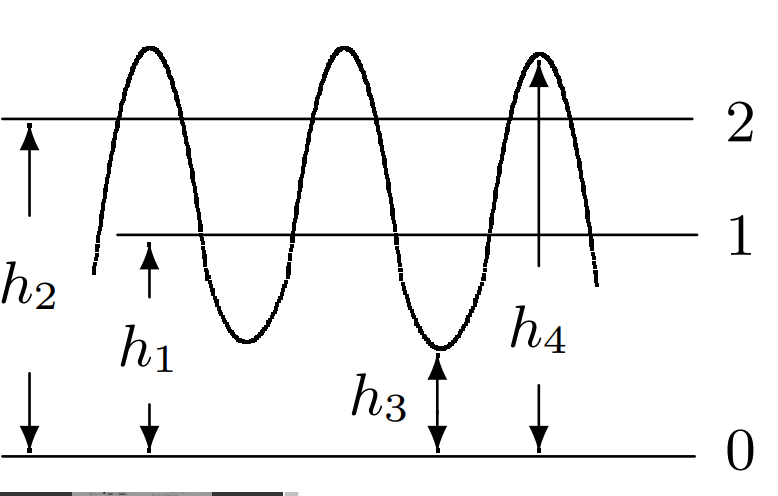
\includegraphics[scale = 0.22]{1.png}
		\caption{Осциллограмма сигналов фотодиода}
		\label{p1}
	\end{center}
\end{figure}
\newpage
Через указанные параметры можно выразить видность $\gamma$ и параметр $\delta$:
\begin{equation}\label{eq:exp}
\delta = \frac{h_1}{h_2} \;(\text{или} \; \frac{h_2}{h_1}); \quad \gamma = \frac{h_4-h_3}{h_4+h_3}
\end{equation}
Измерив величины $h_1$, $h_2$, $h_3$ и $h_4$, можно рассчитать $\gamma$ и $\gamma_1$, а затем определить видность при данной разности хода $l$ для угла между плоскостями поляризации лучей $\alpha = 0$ ($\gamma_3 = 1$):
\[ \gamma_2(l) = \frac{\gamma}{\gamma_1}\]
или при $l = 0$, ($\gamma_2 = 1$) для известного угла $\alpha$:
\[ \gamma_3\left(|\cos{\alpha}|\right) = \frac{\gamma}{\gamma_1}\]

\section{Выполнение}
\subsection{Зависимость видность интерференционной картины от угла поворота поляроида при нулевой разности хода}

Будем сопоставлять две зависимости видности: экспериментальную - $\gamma_3 = \frac{\gamma}{\gamma_1} =  \frac{h_4-h_3}{h_4+h_3} \cdot \frac{2\sqrt{\delta}}{1+\delta} $, где $\delta = \frac{h_1}{h_2}$ и теоретическую - $\gamma_3 = \left(|\cos{\alpha}|\right)$. Получим график: 
\begin{figure}[h!]
	\begin{center}
		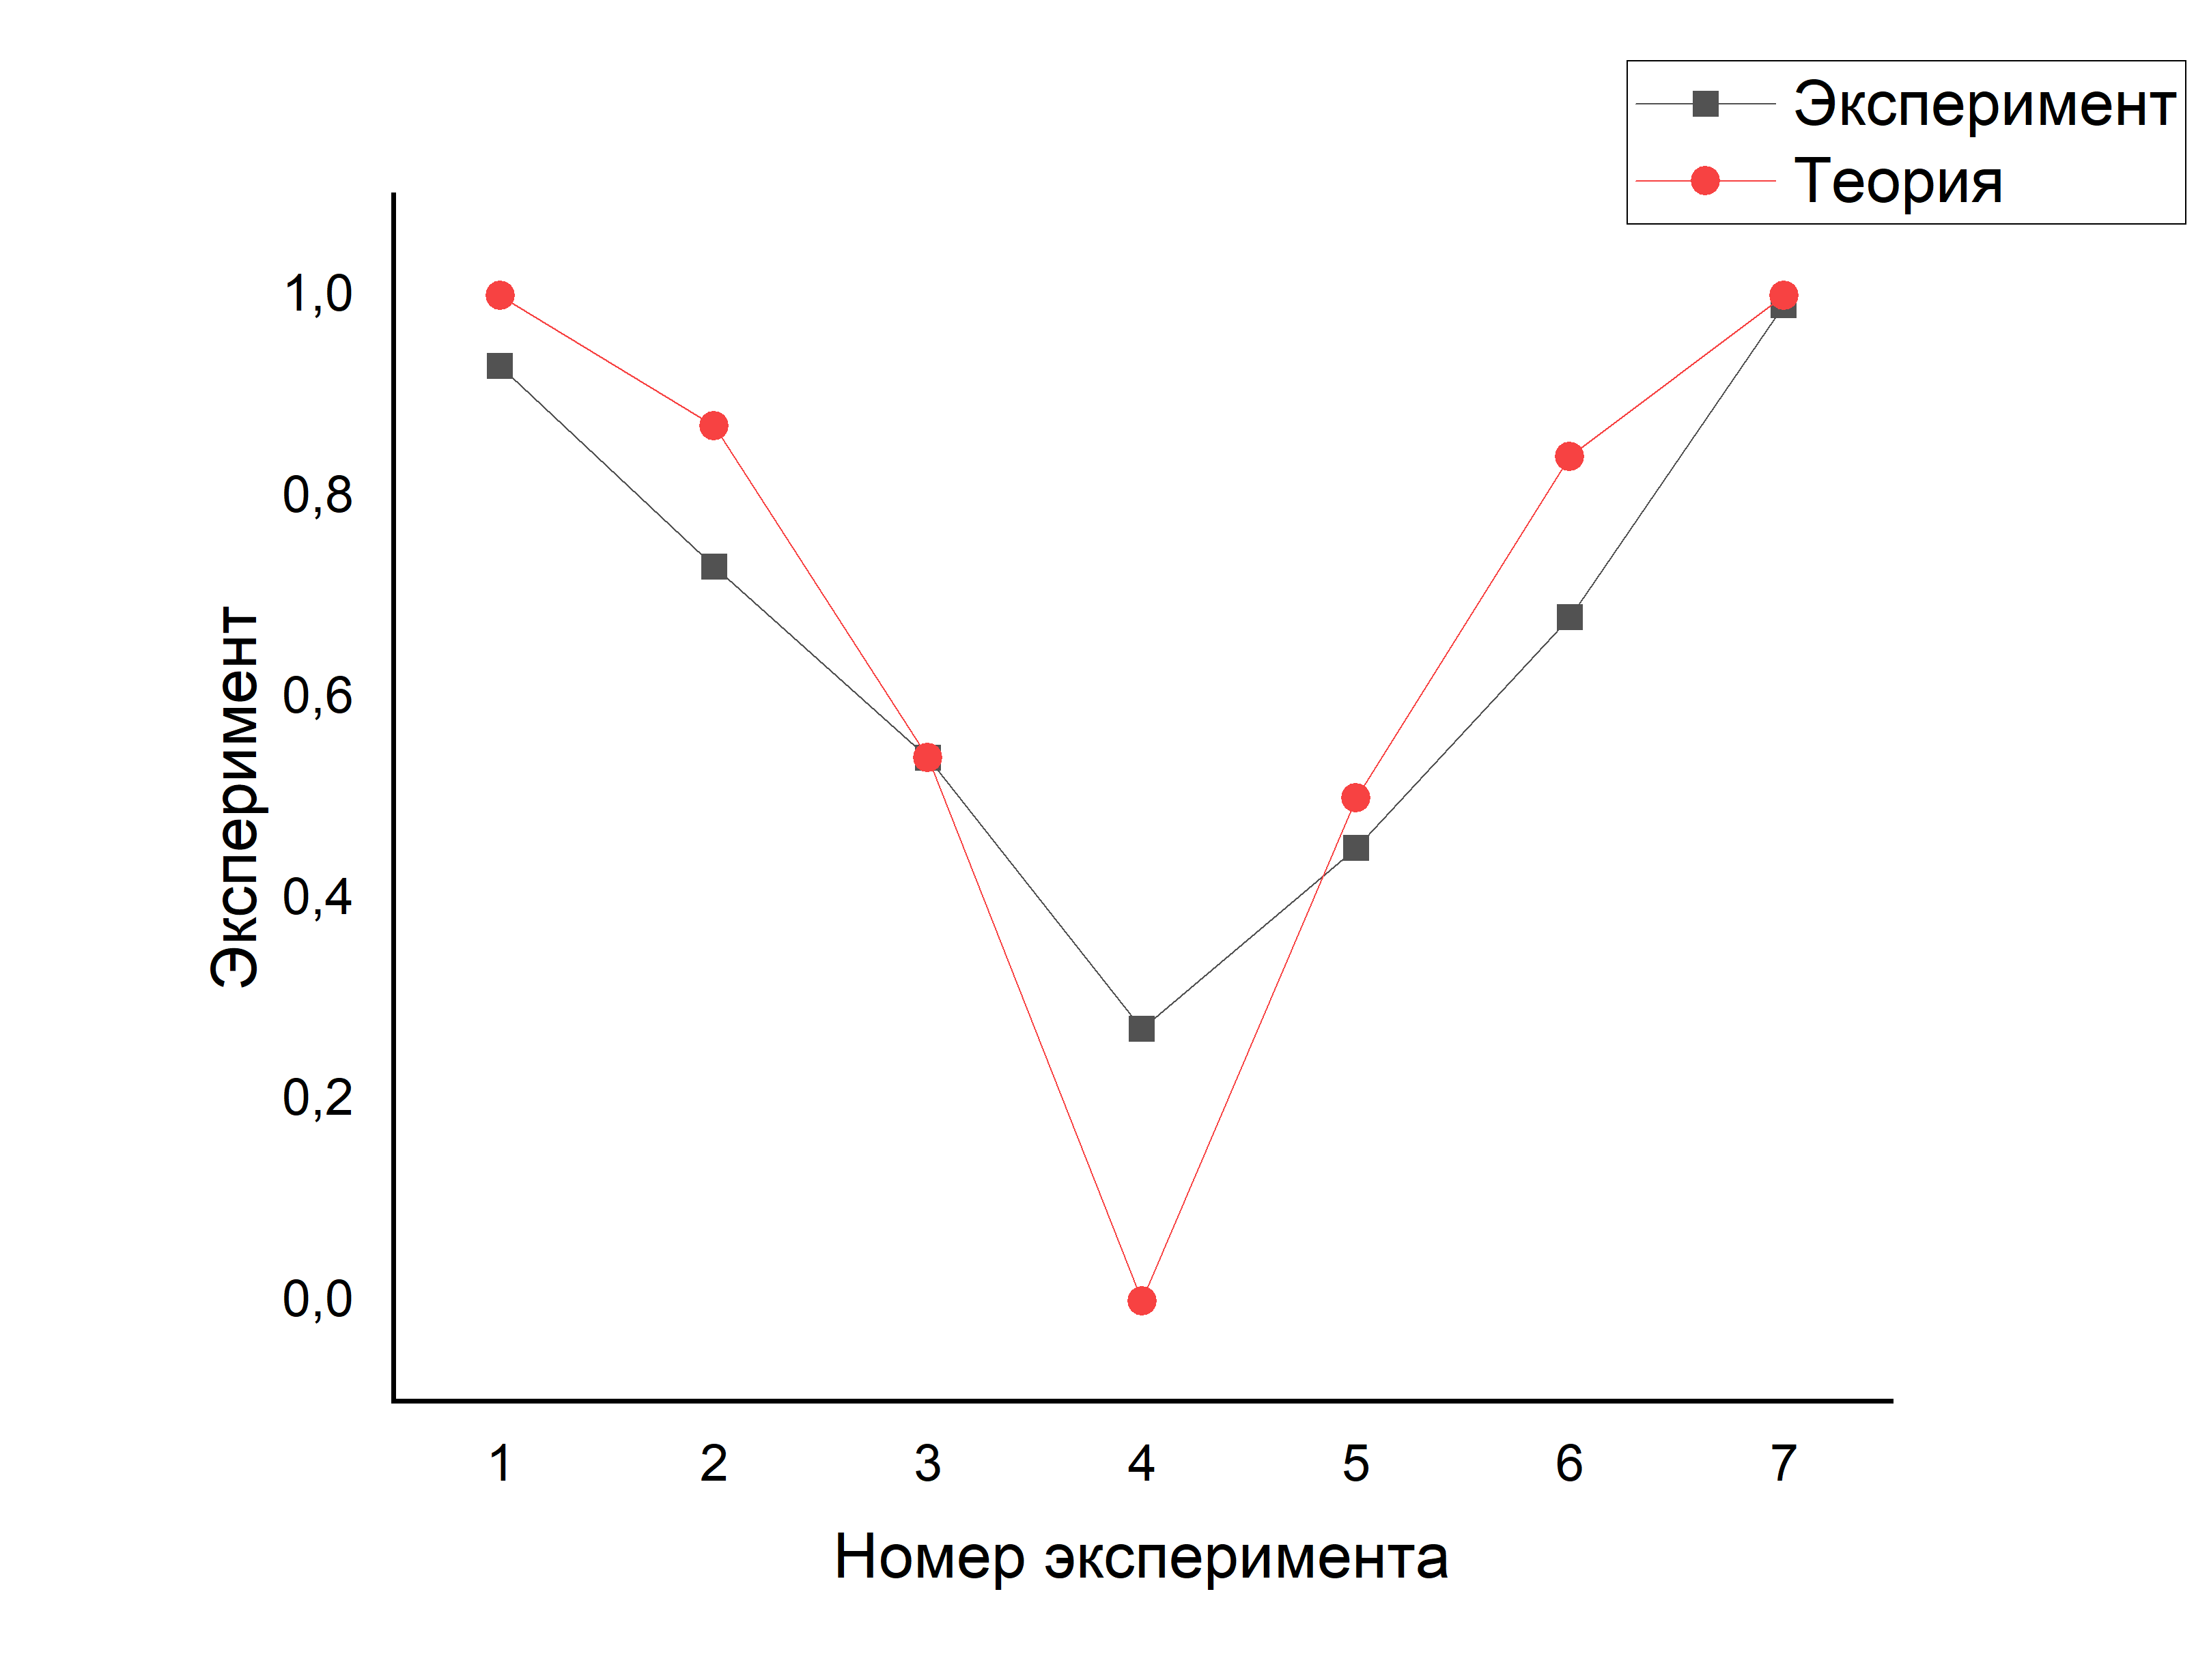
\includegraphics[scale = 0.32]{2.png}
		\caption{Сравнение теории и эксперимента}
		\label{p1}
	\end{center}
\end{figure}
\newpage
Как видим, экспериментальная видность, в отличие от теоретической, не обращается в нуль при определенном значении угла. Это связано с неидеальностью спектра лазера и рассеянием света.

\subsection{Зависимость видности от перемещения зеркала}

Как и в предыдущем пункте, вычисляем экспериментальное значение видности по формуле: $\gamma_2 =  \frac{h_4-h_3}{h_4+h_3} \cdot \frac{2\sqrt{\delta}}{1+\delta} $. Мы получим следующую зависимость от расстояния $L$:

\begin{figure}[h!]
	\begin{center}
		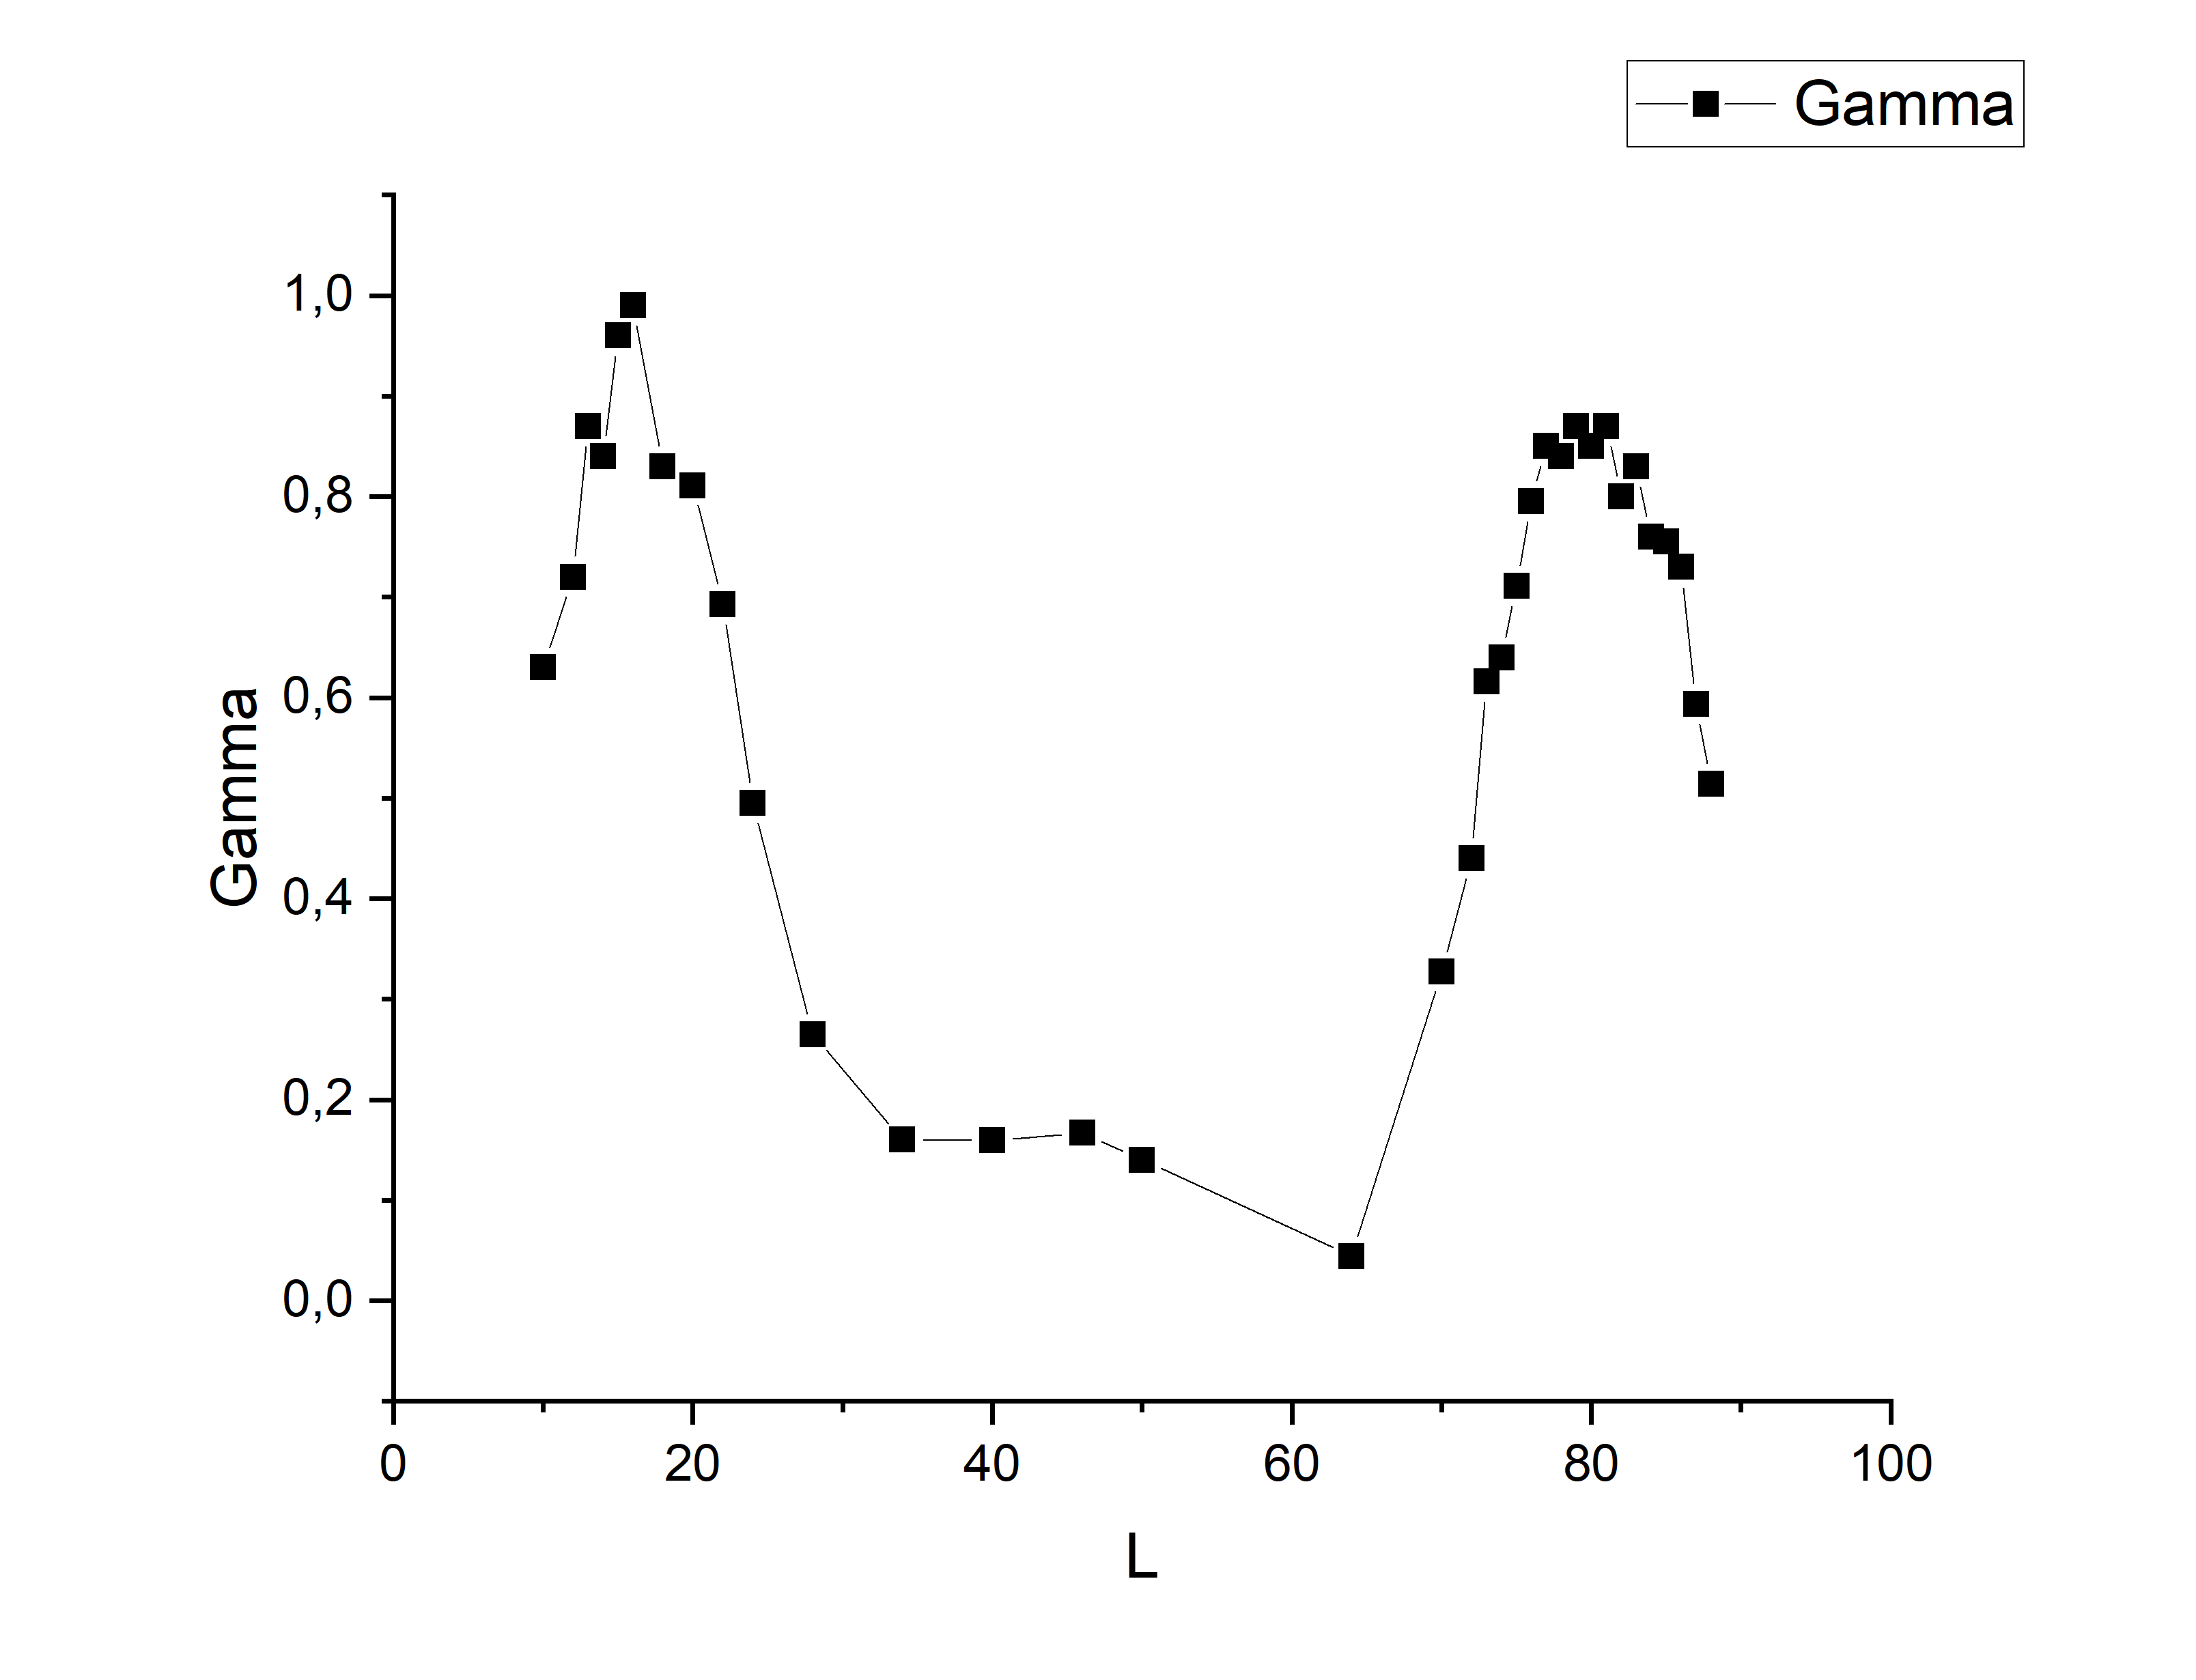
\includegraphics[scale = 0.5]{3.png}
		\caption{Зависимость видность от перемещения зеркала}
		\label{p1}
	\end{center}
\end{figure}
\begin{enumerate}
\item Наблюдаем максимумы по краям области $x_1 \approx (16 \pm 2) \; см \; x_2 \approx (82 \pm 2) \; см $ и некоторые колебания в промежуточной области. \\
Откуда $L = (x_2 - x_1) = (64 \pm 2) \; см$.\\
Межмодовое расстояние: $\varDelta\nu = \frac{c}{2L} \approx (4,5 \pm 0,1)\cdot 10^8 \; Гц$.
\item Определим задержку $l_{1/2}$ на половине высоты главного максимума.\\
$l_{1/2} \approx 6 \pm 2$.
\item Рассчитаем диапазон частот, в котором происходит генерация продольных мод:

\begin{equation}
\varDelta F = \frac{0,6\cdot c}{l_{1/2}} \approx (28,4 \pm 9,7)\cdot 10^8 \; Гц
\end{equation}

\item Оценим число одновременно генерируемых лазером продольных мод:

\begin{equation}
n \approx 1 + \frac{1,2L}{l_{1/2}} \approx 11 \pm 4. 
\end{equation}
\end{enumerate} 
\section{Вывод} 
Была исследована видность интереференционной картины. Рассчитали размер резонатора лазера:  $L = (64 \pm 2) \; см$, межмодовое расстояние $\varDelta\nu = (4,5 \pm 0,1)\cdot 10^8 \; Гц$, диапазон частот, в котором происходит генерация продольных мод $\varDelta F = (12,6 \pm 4,2)\cdot 10^8 \; Гц$, а также оценили число генерируемых лазером продольных мод $	N \approx = 11 \pm 4.$
\end{document} % конец документа